\documentclass[twoside]{book}

% Packages required by doxygen
\usepackage{fixltx2e}
\usepackage{calc}
\usepackage{doxygen}
\usepackage[export]{adjustbox} % also loads graphicx
\usepackage{graphicx}
\usepackage[utf8]{inputenc}
\usepackage{makeidx}
\usepackage{multicol}
\usepackage{multirow}
\PassOptionsToPackage{warn}{textcomp}
\usepackage{textcomp}
\usepackage[nointegrals]{wasysym}
\usepackage[table]{xcolor}

% Font selection
\usepackage[T1]{fontenc}
\usepackage[scaled=.90]{helvet}
\usepackage{courier}
\usepackage{amssymb}
\usepackage{sectsty}
\renewcommand{\familydefault}{\sfdefault}
\allsectionsfont{%
  \fontseries{bc}\selectfont%
  \color{darkgray}%
}
\renewcommand{\DoxyLabelFont}{%
  \fontseries{bc}\selectfont%
  \color{darkgray}%
}
\newcommand{\+}{\discretionary{\mbox{\scriptsize$\hookleftarrow$}}{}{}}

% Page & text layout
\usepackage{geometry}
\geometry{%
  a4paper,%
  top=2.5cm,%
  bottom=2.5cm,%
  left=2.5cm,%
  right=2.5cm%
}
\tolerance=750
\hfuzz=15pt
\hbadness=750
\setlength{\emergencystretch}{15pt}
\setlength{\parindent}{0cm}
\setlength{\parskip}{3ex plus 2ex minus 2ex}
\makeatletter
\renewcommand{\paragraph}{%
  \@startsection{paragraph}{4}{0ex}{-1.0ex}{1.0ex}{%
    \normalfont\normalsize\bfseries\SS@parafont%
  }%
}
\renewcommand{\subparagraph}{%
  \@startsection{subparagraph}{5}{0ex}{-1.0ex}{1.0ex}{%
    \normalfont\normalsize\bfseries\SS@subparafont%
  }%
}
\makeatother

% Headers & footers
\usepackage{fancyhdr}
\pagestyle{fancyplain}
\fancyhead[LE]{\fancyplain{}{\bfseries\thepage}}
\fancyhead[CE]{\fancyplain{}{}}
\fancyhead[RE]{\fancyplain{}{\bfseries\leftmark}}
\fancyhead[LO]{\fancyplain{}{\bfseries\rightmark}}
\fancyhead[CO]{\fancyplain{}{}}
\fancyhead[RO]{\fancyplain{}{\bfseries\thepage}}
\fancyfoot[LE]{\fancyplain{}{}}
\fancyfoot[CE]{\fancyplain{}{}}
\fancyfoot[RE]{\fancyplain{}{\bfseries\scriptsize Generated by Doxygen }}
\fancyfoot[LO]{\fancyplain{}{\bfseries\scriptsize Generated by Doxygen }}
\fancyfoot[CO]{\fancyplain{}{}}
\fancyfoot[RO]{\fancyplain{}{}}
\renewcommand{\footrulewidth}{0.4pt}
\renewcommand{\chaptermark}[1]{%
  \markboth{#1}{}%
}
\renewcommand{\sectionmark}[1]{%
  \markright{\thesection\ #1}%
}

% Indices & bibliography
\usepackage{natbib}
\usepackage[titles]{tocloft}
\setcounter{tocdepth}{3}
\setcounter{secnumdepth}{5}
\makeindex

% Custom commands
\newcommand{\clearemptydoublepage}{%
  \newpage{\pagestyle{empty}\cleardoublepage}%
}

\usepackage{caption}
\captionsetup{labelsep=space,justification=centering,font={bf},singlelinecheck=off,skip=4pt,position=top}

%===== C O N T E N T S =====

\begin{document}

% Titlepage & ToC
\pagenumbering{alph}
\begin{titlepage}
\vspace*{7cm}
\begin{center}%
{\Large Chess End Game \\[1ex]\large Version 1.\+0 }\\
\vspace*{1cm}
{\large Generated by Doxygen 1.8.14}\\
\end{center}
\end{titlepage}
\clearemptydoublepage
\pagenumbering{roman}
\tableofcontents
\clearemptydoublepage
\pagenumbering{arabic}

%--- Begin generated contents ---
\chapter{Hierarchical Index}
\section{Class Hierarchy}
This inheritance list is sorted roughly, but not completely, alphabetically\+:\begin{DoxyCompactList}
\item \contentsline{section}{Chess\+Board}{\pageref{class_chess_board}}{}
\item \contentsline{section}{Chess\+Piece}{\pageref{class_chess_piece}}{}
\begin{DoxyCompactList}
\item \contentsline{section}{King\+Piece}{\pageref{class_king_piece}}{}
\item \contentsline{section}{Rook\+Piece}{\pageref{class_rook_piece}}{}
\end{DoxyCompactList}
\item \contentsline{section}{Position}{\pageref{struct_position}}{}
\end{DoxyCompactList}

\chapter{Class Index}
\section{Class List}
Here are the classes, structs, unions and interfaces with brief descriptions\+:\begin{DoxyCompactList}
\item\contentsline{section}{\textbf{ Chess\+Board} \\*Singleton Board Class }{\pageref{class_chess_board}}{}
\item\contentsline{section}{\textbf{ Chess\+Piece} }{\pageref{class_chess_piece}}{}
\item\contentsline{section}{\textbf{ King\+Piece} }{\pageref{class_king_piece}}{}
\item\contentsline{section}{\textbf{ Position} \\*\doxyref{Position}{p.}{struct_position} on the chess board }{\pageref{struct_position}}{}
\item\contentsline{section}{\textbf{ Rook\+Piece} }{\pageref{class_rook_piece}}{}
\end{DoxyCompactList}

\chapter{File Index}
\section{File List}
Here is a list of all files with brief descriptions\+:\begin{DoxyCompactList}
\item\contentsline{section}{chess\+End\+Game/\textbf{ Chess\+Board.\+cpp} }{\pageref{_chess_board_8cpp}}{}
\item\contentsline{section}{chess\+End\+Game/\textbf{ Chess\+Board.\+hpp} }{\pageref{_chess_board_8hpp}}{}
\item\contentsline{section}{chess\+End\+Game/\textbf{ Chess\+Piece.\+cpp} }{\pageref{_chess_piece_8cpp}}{}
\item\contentsline{section}{chess\+End\+Game/\textbf{ Chess\+Piece.\+hpp} }{\pageref{_chess_piece_8hpp}}{}
\item\contentsline{section}{chess\+End\+Game/\textbf{ Global\+Counter.\+cpp} }{\pageref{_global_counter_8cpp}}{}
\item\contentsline{section}{chess\+End\+Game/\textbf{ Global\+Counter.\+hpp} }{\pageref{_global_counter_8hpp}}{}
\item\contentsline{section}{chess\+End\+Game/\textbf{ King\+Piece.\+cpp} }{\pageref{_king_piece_8cpp}}{}
\item\contentsline{section}{chess\+End\+Game/\textbf{ King\+Piece.\+hpp} }{\pageref{_king_piece_8hpp}}{}
\item\contentsline{section}{chess\+End\+Game/\textbf{ main.\+cpp} }{\pageref{main_8cpp}}{}
\item\contentsline{section}{chess\+End\+Game/\textbf{ Rook\+Piece.\+cpp} }{\pageref{_rook_piece_8cpp}}{}
\item\contentsline{section}{chess\+End\+Game/\textbf{ Rook\+Piece.\+hpp} }{\pageref{_rook_piece_8hpp}}{}
\end{DoxyCompactList}

\chapter{Class Documentation}
\section{Chess\+Board Class Reference}
\label{class_chess_board}\index{Chess\+Board@{Chess\+Board}}


Singleton Board Class.  




{\ttfamily \#include $<$Chess\+Board.\+hpp$>$}

\subsection*{Public Member Functions}
\begin{DoxyCompactItemize}
\item 
\textbf{ Chess\+Board} (\textbf{ Position} a\+\_\+white\+Rook, \textbf{ Position} a\+\_\+white\+King, \textbf{ Position} a\+\_\+black\+King)
\begin{DoxyCompactList}\small\item\em Constructor to initialize a single chessboard. \end{DoxyCompactList}\item 
\textbf{ $\sim$\+Chess\+Board} ()
\begin{DoxyCompactList}\small\item\em Class Deconstructor. \end{DoxyCompactList}\item 
\textbf{ Chess\+Board} $\ast$ \textbf{ get\+Board} (\textbf{ Chess\+Piece} a\+\_\+piece)
\begin{DoxyCompactList}\small\item\em Class Accessors. \end{DoxyCompactList}\item 
bool \textbf{ get\+Piece\+Turn} ()
\item 
\textbf{ Chess\+Piece} $\ast$ \textbf{ get\+Piece} (\textbf{ Position} a\+\_\+cell)
\item 
\textbf{ Position} \textbf{ get\+Piece\+Position} (\textbf{ Piece\+Color} a\+\_\+color, \textbf{ Piece\+Type} a\+\_\+type)
\item 
void \textbf{ set\+Piece} (\textbf{ Position} a\+\_\+cell, \textbf{ Chess\+Piece} $\ast$a\+\_\+piece)
\begin{DoxyCompactList}\small\item\em Class Mutators. \end{DoxyCompactList}\item 
int \textbf{ simulate\+Next\+State} ()
\begin{DoxyCompactList}\small\item\em Next State simulation method -\/ simulates the next state in the chess board. \end{DoxyCompactList}\item 
void \textbf{ display\+Board} ()
\begin{DoxyCompactList}\small\item\em Chess board display method. \end{DoxyCompactList}\item 
void \textbf{ state\+Set\+Piece} (\textbf{ Position} a\+\_\+current, \textbf{ Position} a\+\_\+dest)
\begin{DoxyCompactList}\small\item\em Sets chess piece for states. \end{DoxyCompactList}\item 
int \textbf{ corner\+Black\+King} (\textbf{ Chess\+Board} $\ast$a\+\_\+node)
\begin{DoxyCompactList}\small\item\em Heuristic for minimax algorithm. \end{DoxyCompactList}\item 
int \textbf{ minimax} (\textbf{ Chess\+Board} $\ast$a\+\_\+node, int a\+\_\+depth, int a\+\_\+alpha, int a\+\_\+beta, bool a\+\_\+color, int \&a\+\_\+count)
\begin{DoxyCompactList}\small\item\em Implementation of minimax algorithm with alpha beta pruning. \end{DoxyCompactList}\item 
void \textbf{ write\+Results} (\textbf{ Piece\+Color} a\+\_\+type)
\begin{DoxyCompactList}\small\item\em Method to write the final results to the result file. \end{DoxyCompactList}\end{DoxyCompactItemize}
\subsection*{Private Member Functions}
\begin{DoxyCompactItemize}
\item 
void \textbf{ move\+Piece} (bool a\+\_\+piece\+Turn)
\begin{DoxyCompactList}\small\item\em Move Chess Piece of the passed color. \end{DoxyCompactList}\end{DoxyCompactItemize}
\subsection*{Private Attributes}
\begin{DoxyCompactItemize}
\item 
\textbf{ Chess\+Board} $\ast$ \textbf{ m\+\_\+game\+Instance}
\item 
\textbf{ Chess\+Piece} $\ast$ \textbf{ m\+\_\+chess\+Grid} [8][8]
\begin{DoxyCompactList}\small\item\em Chessboard grid where the game is played. \end{DoxyCompactList}\item 
\textbf{ King\+Piece} $\ast$ \textbf{ m\+\_\+white\+King\+Piece}
\begin{DoxyCompactList}\small\item\em Chess pieces. \end{DoxyCompactList}\item 
\textbf{ King\+Piece} $\ast$ \textbf{ m\+\_\+black\+King\+Piece}
\item 
\textbf{ Rook\+Piece} $\ast$ \textbf{ m\+\_\+white\+Rook\+Piece}
\item 
bool \textbf{ m\+\_\+piece\+Turn} = 1
\item 
int \textbf{ count}
\begin{DoxyCompactList}\small\item\em Counter for number of steps in the game. \end{DoxyCompactList}\end{DoxyCompactItemize}


\subsection{Detailed Description}
Singleton Board Class. 

\subsection{Constructor \& Destructor Documentation}
\mbox{\label{class_chess_board_a7e1515e731f1cc05910ecd77ed9ddbfe}} 
\index{Chess\+Board@{Chess\+Board}!Chess\+Board@{Chess\+Board}}
\index{Chess\+Board@{Chess\+Board}!Chess\+Board@{Chess\+Board}}
\subsubsection{Chess\+Board()}
{\footnotesize\ttfamily Chess\+Board\+::\+Chess\+Board (\begin{DoxyParamCaption}\item[{\textbf{ Position}}]{a\+\_\+white\+Rook,  }\item[{\textbf{ Position}}]{a\+\_\+white\+King,  }\item[{\textbf{ Position}}]{a\+\_\+black\+King }\end{DoxyParamCaption})}



Constructor to initialize a single chessboard. 

Constructor for the \doxyref{Chess\+Board}{p.}{class_chess_board} class. Takes position of White Rook, White King, and Black King to construct a Chess board environment. 
\begin{DoxyParams}{Parameters}
{\em a\+\_\+white\+Rook} & \doxyref{Position}{p.}{struct_position} Initial position of the White Rook. \\
\hline
{\em a\+\_\+white\+King} & \doxyref{Position}{p.}{struct_position} Initial position of the White King. \\
\hline
{\em a\+\_\+black\+King} & Initial position of the Black King. \\
\hline
\end{DoxyParams}
\begin{DoxySeeAlso}{See also}
\doxyref{Rook\+Piece}{p.}{class_rook_piece} and \doxyref{King\+Piece}{p.}{class_king_piece} constructors. 
\end{DoxySeeAlso}
\mbox{\label{class_chess_board_acece8633f444b90d7b371b57f52d0780}} 
\index{Chess\+Board@{Chess\+Board}!````~Chess\+Board@{$\sim$\+Chess\+Board}}
\index{````~Chess\+Board@{$\sim$\+Chess\+Board}!Chess\+Board@{Chess\+Board}}
\subsubsection{$\sim$\+Chess\+Board()}
{\footnotesize\ttfamily Chess\+Board\+::$\sim$\+Chess\+Board (\begin{DoxyParamCaption}{ }\end{DoxyParamCaption})}



Class Deconstructor. 

\doxyref{Chess\+Board}{p.}{class_chess_board} Class Deconstructor Frees dynamically allocated memory for the players in the game. 

\subsection{Member Function Documentation}
\mbox{\label{class_chess_board_a889a2c4d8162c791898d59df2dcc54b0}} 
\index{Chess\+Board@{Chess\+Board}!corner\+Black\+King@{corner\+Black\+King}}
\index{corner\+Black\+King@{corner\+Black\+King}!Chess\+Board@{Chess\+Board}}
\subsubsection{corner\+Black\+King()}
{\footnotesize\ttfamily int Chess\+Board\+::corner\+Black\+King (\begin{DoxyParamCaption}\item[{\textbf{ Chess\+Board} $\ast$}]{a\+\_\+node }\end{DoxyParamCaption})}



Heuristic for minimax algorithm. 

Heuristic method to corner the Black King. Used by the white pieces for the minimax alpha-\/beta pruned algorithm 
\begin{DoxyParams}{Parameters}
{\em a\+\_\+node} & Chess\+Board$\ast$ The current state of the board. \\
\hline
\end{DoxyParams}
\begin{DoxyReturn}{Returns}
int The score for the state according to the heuristics. 
\end{DoxyReturn}
\mbox{\label{class_chess_board_af3e74d5a4bc99fc55676c660ce71b60f}} 
\index{Chess\+Board@{Chess\+Board}!display\+Board@{display\+Board}}
\index{display\+Board@{display\+Board}!Chess\+Board@{Chess\+Board}}
\subsubsection{display\+Board()}
{\footnotesize\ttfamily void Chess\+Board\+::display\+Board (\begin{DoxyParamCaption}{ }\end{DoxyParamCaption})}



Chess board display method. 

Method to display chess board. Displays the chess board as a character grid. Additionally writes the end game configurations to a text file with the result of the match. \mbox{\label{class_chess_board_ab71c884798ec4694ef363eefd6f5adea}} 
\index{Chess\+Board@{Chess\+Board}!get\+Board@{get\+Board}}
\index{get\+Board@{get\+Board}!Chess\+Board@{Chess\+Board}}
\subsubsection{get\+Board()}
{\footnotesize\ttfamily \textbf{ Chess\+Board}$\ast$ Chess\+Board\+::get\+Board (\begin{DoxyParamCaption}\item[{\textbf{ Chess\+Piece}}]{a\+\_\+piece }\end{DoxyParamCaption})\hspace{0.3cm}{\ttfamily [inline]}}



Class Accessors. 

\mbox{\label{class_chess_board_a610d3d12ab9cdf0560f533c73a89bef1}} 
\index{Chess\+Board@{Chess\+Board}!get\+Piece@{get\+Piece}}
\index{get\+Piece@{get\+Piece}!Chess\+Board@{Chess\+Board}}
\subsubsection{get\+Piece()}
{\footnotesize\ttfamily \textbf{ Chess\+Piece} $\ast$ Chess\+Board\+::get\+Piece (\begin{DoxyParamCaption}\item[{\textbf{ Position}}]{a\+\_\+cell }\end{DoxyParamCaption})}

Accessor method to get chess piece on a board position. Gets chess piece at position a\+\_\+cell. 
\begin{DoxyParams}{Parameters}
{\em a\+\_\+cell} & \doxyref{Position}{p.}{struct_position} (x, y) position of the chess piece. \\
\hline
\end{DoxyParams}
\begin{DoxyReturn}{Returns}
Chess\+Piece$\ast$ \doxyref{Chess\+Piece}{p.}{class_chess_piece} in position (x,y) 
\end{DoxyReturn}
\mbox{\label{class_chess_board_a72fd59742d446ada232cf2bf30f1f5bd}} 
\index{Chess\+Board@{Chess\+Board}!get\+Piece\+Position@{get\+Piece\+Position}}
\index{get\+Piece\+Position@{get\+Piece\+Position}!Chess\+Board@{Chess\+Board}}
\subsubsection{get\+Piece\+Position()}
{\footnotesize\ttfamily \textbf{ Position} Chess\+Board\+::get\+Piece\+Position (\begin{DoxyParamCaption}\item[{\textbf{ Piece\+Color}}]{a\+\_\+color,  }\item[{\textbf{ Piece\+Type}}]{a\+\_\+type }\end{DoxyParamCaption})}

Accessor method to get the possition of a chess piece on the board. Gets position of a particular type and color. 
\begin{DoxyParams}{Parameters}
{\em a\+\_\+color} & Piece\+Color The color of the chess piece. \\
\hline
{\em a\+\_\+type} & Piece\+Type The type of the chess piece. \\
\hline
\end{DoxyParams}
\begin{DoxyReturn}{Returns}
\doxyref{Position}{p.}{struct_position} The position of the chess piece. 
\end{DoxyReturn}
\mbox{\label{class_chess_board_ab10cc089b3e4504cfe74fb3e6ab9f830}} 
\index{Chess\+Board@{Chess\+Board}!get\+Piece\+Turn@{get\+Piece\+Turn}}
\index{get\+Piece\+Turn@{get\+Piece\+Turn}!Chess\+Board@{Chess\+Board}}
\subsubsection{get\+Piece\+Turn()}
{\footnotesize\ttfamily bool Chess\+Board\+::get\+Piece\+Turn (\begin{DoxyParamCaption}{ }\end{DoxyParamCaption})\hspace{0.3cm}{\ttfamily [inline]}}

\mbox{\label{class_chess_board_a1a27f7cbe73d1fe3dc3ea79501e8cb25}} 
\index{Chess\+Board@{Chess\+Board}!minimax@{minimax}}
\index{minimax@{minimax}!Chess\+Board@{Chess\+Board}}
\subsubsection{minimax()}
{\footnotesize\ttfamily int Chess\+Board\+::minimax (\begin{DoxyParamCaption}\item[{\textbf{ Chess\+Board} $\ast$}]{a\+\_\+node,  }\item[{int}]{a\+\_\+depth,  }\item[{int}]{a\+\_\+alpha,  }\item[{int}]{a\+\_\+beta,  }\item[{bool}]{a\+\_\+color,  }\item[{int \&}]{a\+\_\+count }\end{DoxyParamCaption})}



Implementation of minimax algorithm with alpha beta pruning. 

Minimax algorithm implementation with alpha beta pruning. Used by white pieces to get the optimal next move. 
\begin{DoxyParams}{Parameters}
{\em a\+\_\+node} & Chess\+Board$\ast$ The current state of the board. \\
\hline
{\em a\+\_\+depth} & int The depth to search for the optimal state. \\
\hline
{\em a\+\_\+alpha} & int alpha cut off. \\
\hline
{\em a\+\_\+beta} & int beta cut off. \\
\hline
{\em a\+\_\+color} & bool The current piece color \\
\hline
{\em a\+\_\+count} & int Counter for the number of states \\
\hline
\end{DoxyParams}
\begin{DoxyReturn}{Returns}
int The score for the state according to the heuristics. 
\end{DoxyReturn}
\mbox{\label{class_chess_board_a98c46e36d99053d46de330f94f72716f}} 
\index{Chess\+Board@{Chess\+Board}!move\+Piece@{move\+Piece}}
\index{move\+Piece@{move\+Piece}!Chess\+Board@{Chess\+Board}}
\subsubsection{move\+Piece()}
{\footnotesize\ttfamily void Chess\+Board\+::move\+Piece (\begin{DoxyParamCaption}\item[{bool}]{a\+\_\+piece\+Turn }\end{DoxyParamCaption})\hspace{0.3cm}{\ttfamily [private]}}



Move Chess Piece of the passed color. 

\mbox{\label{class_chess_board_a427021f34895ac47cb6ba8aacf921663}} 
\index{Chess\+Board@{Chess\+Board}!set\+Piece@{set\+Piece}}
\index{set\+Piece@{set\+Piece}!Chess\+Board@{Chess\+Board}}
\subsubsection{set\+Piece()}
{\footnotesize\ttfamily void Chess\+Board\+::set\+Piece (\begin{DoxyParamCaption}\item[{\textbf{ Position}}]{a\+\_\+cell,  }\item[{\textbf{ Chess\+Piece} $\ast$}]{a\+\_\+piece }\end{DoxyParamCaption})}



Class Mutators. 

Mutator method to set chess piece on a board position. Sets chess piece a\+\_\+piece at position (x,y). 
\begin{DoxyParams}{Parameters}
{\em a\+\_\+cell} & \doxyref{Position}{p.}{struct_position} (x, y) position to put the chess piece. \\
\hline
{\em a\+\_\+piece} & Chess\+Piece$\ast$ Agent to place in position (x,y) \\
\hline
\end{DoxyParams}
\mbox{\label{class_chess_board_a6d0ddb591893d37452d5c3b90efab4da}} 
\index{Chess\+Board@{Chess\+Board}!simulate\+Next\+State@{simulate\+Next\+State}}
\index{simulate\+Next\+State@{simulate\+Next\+State}!Chess\+Board@{Chess\+Board}}
\subsubsection{simulate\+Next\+State()}
{\footnotesize\ttfamily int Chess\+Board\+::simulate\+Next\+State (\begin{DoxyParamCaption}{ }\end{DoxyParamCaption})}



Next State simulation method -\/ simulates the next state in the chess board. 

Next State simulation method. Simulates the next state on the chess board. \begin{DoxyReturn}{Returns}
int Returns 1 when the game ends due to checkmate and 2 when draw. 0 when in progress. 
\end{DoxyReturn}
\mbox{\label{class_chess_board_aab31a05caf521f36ae6d0a726b6fe13e}} 
\index{Chess\+Board@{Chess\+Board}!state\+Set\+Piece@{state\+Set\+Piece}}
\index{state\+Set\+Piece@{state\+Set\+Piece}!Chess\+Board@{Chess\+Board}}
\subsubsection{state\+Set\+Piece()}
{\footnotesize\ttfamily void Chess\+Board\+::state\+Set\+Piece (\begin{DoxyParamCaption}\item[{\textbf{ Position}}]{a\+\_\+current,  }\item[{\textbf{ Position}}]{a\+\_\+dest }\end{DoxyParamCaption})}



Sets chess piece for states. 

Method to create states for minimax and greedy algorithn. Sets chess piece for the states created from current position to destination position. 
\begin{DoxyParams}{Parameters}
{\em a\+\_\+current} & \doxyref{Position}{p.}{struct_position} Current position of the piece \\
\hline
{\em a\+\_\+dest} & \doxyref{Position}{p.}{struct_position} Destination position of the piece \\
\hline
\end{DoxyParams}
\mbox{\label{class_chess_board_a92c39020cf378c89590883e943cb7131}} 
\index{Chess\+Board@{Chess\+Board}!write\+Results@{write\+Results}}
\index{write\+Results@{write\+Results}!Chess\+Board@{Chess\+Board}}
\subsubsection{write\+Results()}
{\footnotesize\ttfamily void Chess\+Board\+::write\+Results (\begin{DoxyParamCaption}\item[{\textbf{ Piece\+Color}}]{a\+\_\+type }\end{DoxyParamCaption})}



Method to write the final results to the result file. 

Method to write the end game configurations to a target file. Writes the piece position, the outcome of the game and the statistics of the game. 
\begin{DoxyParams}{Parameters}
{\em a\+\_\+type} & The color who won the game. Black color signifies a draw. \\
\hline
\end{DoxyParams}


\subsection{Member Data Documentation}
\mbox{\label{class_chess_board_a41517b6a4f2136639dc42f047da069ef}} 
\index{Chess\+Board@{Chess\+Board}!count@{count}}
\index{count@{count}!Chess\+Board@{Chess\+Board}}
\subsubsection{count}
{\footnotesize\ttfamily int Chess\+Board\+::count\hspace{0.3cm}{\ttfamily [private]}}



Counter for number of steps in the game. 

\mbox{\label{class_chess_board_ab4d77245ab3d6e35caa3dfff55354096}} 
\index{Chess\+Board@{Chess\+Board}!m\+\_\+black\+King\+Piece@{m\+\_\+black\+King\+Piece}}
\index{m\+\_\+black\+King\+Piece@{m\+\_\+black\+King\+Piece}!Chess\+Board@{Chess\+Board}}
\subsubsection{m\+\_\+black\+King\+Piece}
{\footnotesize\ttfamily \textbf{ King\+Piece}$\ast$ Chess\+Board\+::m\+\_\+black\+King\+Piece\hspace{0.3cm}{\ttfamily [private]}}

\mbox{\label{class_chess_board_aef98e86c15b207f04d7d275773753c71}} 
\index{Chess\+Board@{Chess\+Board}!m\+\_\+chess\+Grid@{m\+\_\+chess\+Grid}}
\index{m\+\_\+chess\+Grid@{m\+\_\+chess\+Grid}!Chess\+Board@{Chess\+Board}}
\subsubsection{m\+\_\+chess\+Grid}
{\footnotesize\ttfamily \textbf{ Chess\+Piece}$\ast$ Chess\+Board\+::m\+\_\+chess\+Grid[8][8]\hspace{0.3cm}{\ttfamily [private]}}



Chessboard grid where the game is played. 

\mbox{\label{class_chess_board_aaa31b798b70fa50d3469939d9acd0924}} 
\index{Chess\+Board@{Chess\+Board}!m\+\_\+game\+Instance@{m\+\_\+game\+Instance}}
\index{m\+\_\+game\+Instance@{m\+\_\+game\+Instance}!Chess\+Board@{Chess\+Board}}
\subsubsection{m\+\_\+game\+Instance}
{\footnotesize\ttfamily \textbf{ Chess\+Board}$\ast$ Chess\+Board\+::m\+\_\+game\+Instance\hspace{0.3cm}{\ttfamily [private]}}

C\+H\+E\+SS G\+A\+ME V\+A\+R\+I\+A\+B\+L\+ES\+: Variable to hold the game instance. \mbox{\label{class_chess_board_aa553379321272c4fee083a23a78a85c1}} 
\index{Chess\+Board@{Chess\+Board}!m\+\_\+piece\+Turn@{m\+\_\+piece\+Turn}}
\index{m\+\_\+piece\+Turn@{m\+\_\+piece\+Turn}!Chess\+Board@{Chess\+Board}}
\subsubsection{m\+\_\+piece\+Turn}
{\footnotesize\ttfamily bool Chess\+Board\+::m\+\_\+piece\+Turn = 1\hspace{0.3cm}{\ttfamily [private]}}

Bool to hold color turn 1 for White and 0 for Black. Game starts with white\textquotesingle{}s move. \mbox{\label{class_chess_board_a97a4f8f8af24f24d2975d69fbe8f9834}} 
\index{Chess\+Board@{Chess\+Board}!m\+\_\+white\+King\+Piece@{m\+\_\+white\+King\+Piece}}
\index{m\+\_\+white\+King\+Piece@{m\+\_\+white\+King\+Piece}!Chess\+Board@{Chess\+Board}}
\subsubsection{m\+\_\+white\+King\+Piece}
{\footnotesize\ttfamily \textbf{ King\+Piece}$\ast$ Chess\+Board\+::m\+\_\+white\+King\+Piece\hspace{0.3cm}{\ttfamily [private]}}



Chess pieces. 

\mbox{\label{class_chess_board_a43776b52aa4db67366b70c7dd369a97d}} 
\index{Chess\+Board@{Chess\+Board}!m\+\_\+white\+Rook\+Piece@{m\+\_\+white\+Rook\+Piece}}
\index{m\+\_\+white\+Rook\+Piece@{m\+\_\+white\+Rook\+Piece}!Chess\+Board@{Chess\+Board}}
\subsubsection{m\+\_\+white\+Rook\+Piece}
{\footnotesize\ttfamily \textbf{ Rook\+Piece}$\ast$ Chess\+Board\+::m\+\_\+white\+Rook\+Piece\hspace{0.3cm}{\ttfamily [private]}}



The documentation for this class was generated from the following files\+:\begin{DoxyCompactItemize}
\item 
chess\+End\+Game/\textbf{ Chess\+Board.\+hpp}\item 
chess\+End\+Game/\textbf{ Chess\+Board.\+cpp}\end{DoxyCompactItemize}

\section{Chess\+Piece Class Reference}
\label{class_chess_piece}\index{Chess\+Piece@{Chess\+Piece}}


{\ttfamily \#include $<$Chess\+Piece.\+hpp$>$}

Inheritance diagram for Chess\+Piece\+:\begin{figure}[H]
\begin{center}
\leavevmode
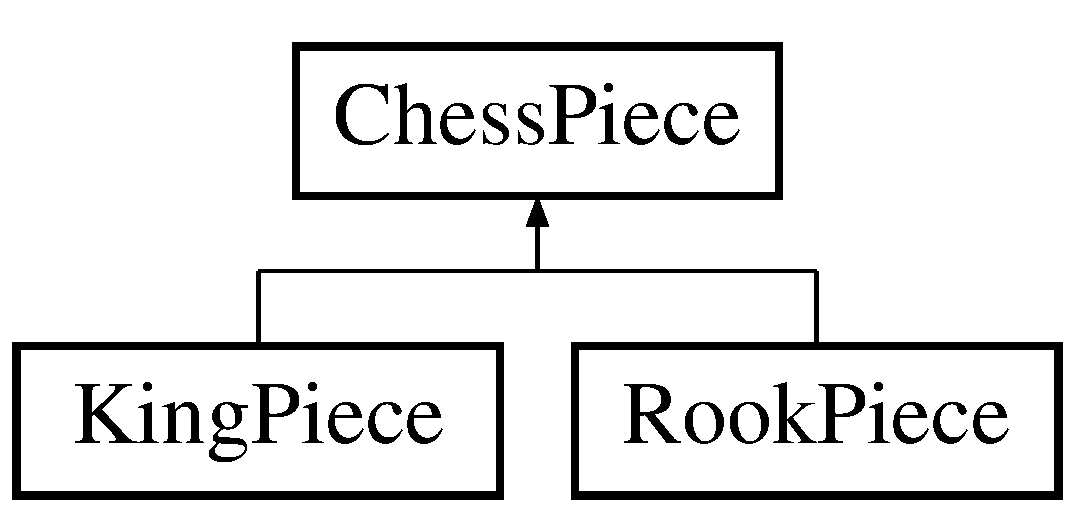
\includegraphics[height=2.000000cm]{class_chess_piece}
\end{center}
\end{figure}
\subsection*{Public Member Functions}
\begin{DoxyCompactItemize}
\item 
\textbf{ Chess\+Piece} (class \textbf{ Chess\+Board} $\ast$a\+\_\+board, \textbf{ Position} a\+\_\+cell, \textbf{ Piece\+Color} a\+\_\+piece\+Color)
\begin{DoxyCompactList}\small\item\em \doxyref{Chess\+Piece}{p.}{class_chess_piece} constructor -\/ Creates a chess piece in the chess board at passed position. \end{DoxyCompactList}\item 
virtual \textbf{ $\sim$\+Chess\+Piece} ()
\begin{DoxyCompactList}\small\item\em \doxyref{Chess\+Piece}{p.}{class_chess_piece} destructor. \end{DoxyCompactList}\item 
virtual int \textbf{ move\+Piece} ()=0
\begin{DoxyCompactList}\small\item\em Moves the chess piece on the board. \end{DoxyCompactList}\item 
virtual \textbf{ Piece\+Type} \textbf{ get\+Piece\+Type} ()=0
\item 
\textbf{ Position} \textbf{ get\+Piece\+Position} ()
\begin{DoxyCompactList}\small\item\em Get Piece \doxyref{Position}{p.}{struct_position}. \end{DoxyCompactList}\item 
virtual char \textbf{ piece\+Char\+Code} ()=0
\begin{DoxyCompactList}\small\item\em Get character representation of the chess piece. \end{DoxyCompactList}\item 
char \textbf{ piece\+Color\+Code} ()
\begin{DoxyCompactList}\small\item\em Get color representation of the chess piece. \end{DoxyCompactList}\item 
bool \textbf{ check\+Cell} (\textbf{ Position} a\+\_\+cell)
\begin{DoxyCompactList}\small\item\em Validate cell is on the board. \end{DoxyCompactList}\item 
virtual std\+::vector$<$ \textbf{ Position} $>$ \textbf{ get\+Possible\+Moves} ()=0
\begin{DoxyCompactList}\small\item\em Get possible moves for the chess piece. \end{DoxyCompactList}\item 
int \textbf{ get\+Maximizing\+State} (\textbf{ Position} \&a\+\_\+pos)
\begin{DoxyCompactList}\small\item\em Gets the maximizing state for the chess piece. \end{DoxyCompactList}\item 
void \textbf{ update\+Piece\+Cell} (\textbf{ Position} a\+\_\+cell)
\begin{DoxyCompactList}\small\item\em Moves chess piece to new position (x, y) \end{DoxyCompactList}\end{DoxyCompactItemize}
\subsection*{Protected Attributes}
\begin{DoxyCompactItemize}
\item 
\textbf{ Position} \textbf{ m\+\_\+piece\+Position}
\begin{DoxyCompactList}\small\item\em Variable that holds the position of a chess piece. \end{DoxyCompactList}\item 
\textbf{ Chess\+Board} $\ast$ \textbf{ m\+\_\+board}
\begin{DoxyCompactList}\small\item\em Pointer to the chess board. \end{DoxyCompactList}\item 
\textbf{ Piece\+Color} \textbf{ m\+\_\+piece\+Color}
\begin{DoxyCompactList}\small\item\em Variable that holds the color of the chess piece. \end{DoxyCompactList}\end{DoxyCompactItemize}


\subsection{Constructor \& Destructor Documentation}
\mbox{\label{class_chess_piece_a2d766e242cffc9d4dec12ba4be5eb871}} 
\index{Chess\+Piece@{Chess\+Piece}!Chess\+Piece@{Chess\+Piece}}
\index{Chess\+Piece@{Chess\+Piece}!Chess\+Piece@{Chess\+Piece}}
\subsubsection{Chess\+Piece()}
{\footnotesize\ttfamily Chess\+Piece\+::\+Chess\+Piece (\begin{DoxyParamCaption}\item[{class \textbf{ Chess\+Board} $\ast$}]{a\+\_\+board,  }\item[{\textbf{ Position}}]{a\+\_\+cell,  }\item[{\textbf{ Piece\+Color}}]{a\+\_\+piece\+Color }\end{DoxyParamCaption})}



\doxyref{Chess\+Piece}{p.}{class_chess_piece} constructor -\/ Creates a chess piece in the chess board at passed position. 

\doxyref{Chess\+Piece.\+cpp}{p.}{_chess_piece_8cpp} Implementation of \doxyref{Chess\+Piece.\+hpp}{p.}{_chess_piece_8hpp} class.

Created by Salil D. Maharjan on 11/27/19. Copyright © 2019 Salil Maharjan. All rights reserved. Constructor for \doxyref{Chess\+Piece}{p.}{class_chess_piece} Class. Constructor\+: Creates a chess piece on the board at position (x,y) 
\begin{DoxyParams}{Parameters}
{\em a\+\_\+board} & Chess\+Board$\ast$ Board where the game is being played. \\
\hline
{\em a\+\_\+cell} & \doxyref{Position}{p.}{struct_position} (x,y) position in the board. \\
\hline
{\em a\+\_\+piece\+Color} & Piece\+Color Chess Piece Color. \\
\hline
\end{DoxyParams}
\mbox{\label{class_chess_piece_a55fa05bb289888ca0ff5895a6f155960}} 
\index{Chess\+Piece@{Chess\+Piece}!````~Chess\+Piece@{$\sim$\+Chess\+Piece}}
\index{````~Chess\+Piece@{$\sim$\+Chess\+Piece}!Chess\+Piece@{Chess\+Piece}}
\subsubsection{$\sim$\+Chess\+Piece()}
{\footnotesize\ttfamily Chess\+Piece\+::$\sim$\+Chess\+Piece (\begin{DoxyParamCaption}{ }\end{DoxyParamCaption})\hspace{0.3cm}{\ttfamily [virtual]}}



\doxyref{Chess\+Piece}{p.}{class_chess_piece} destructor. 

Empty Destructor for \doxyref{Chess\+Piece}{p.}{class_chess_piece} class. 

\subsection{Member Function Documentation}
\mbox{\label{class_chess_piece_a439fb5b59088169611c415b33d6f3510}} 
\index{Chess\+Piece@{Chess\+Piece}!check\+Cell@{check\+Cell}}
\index{check\+Cell@{check\+Cell}!Chess\+Piece@{Chess\+Piece}}
\subsubsection{check\+Cell()}
{\footnotesize\ttfamily bool Chess\+Piece\+::check\+Cell (\begin{DoxyParamCaption}\item[{\textbf{ Position}}]{a\+\_\+cell }\end{DoxyParamCaption})}



Validate cell is on the board. 

Method to check if cell is in range. Checks if a position is in the board or out of range. 
\begin{DoxyParams}{Parameters}
{\em a\+\_\+cell} & \doxyref{Position}{p.}{struct_position} (x,y) position in the board. \\
\hline
\end{DoxyParams}
\begin{DoxyReturn}{Returns}
bool if \doxyref{Position}{p.}{struct_position} (x,y) is in the board. 
\end{DoxyReturn}
\mbox{\label{class_chess_piece_af8037e1f83f287884586588948bc478e}} 
\index{Chess\+Piece@{Chess\+Piece}!get\+Maximizing\+State@{get\+Maximizing\+State}}
\index{get\+Maximizing\+State@{get\+Maximizing\+State}!Chess\+Piece@{Chess\+Piece}}
\subsubsection{get\+Maximizing\+State()}
{\footnotesize\ttfamily int Chess\+Piece\+::get\+Maximizing\+State (\begin{DoxyParamCaption}\item[{\textbf{ Position} \&}]{a\+\_\+pos }\end{DoxyParamCaption})}



Gets the maximizing state for the chess piece. 

Method to get the maximizing state for a chess piece. 
\begin{DoxyParams}{Parameters}
{\em a\+\_\+pos} & \doxyref{Position}{p.}{struct_position} (x,y) position on the board passeed by reference. The position is updated with the maximizing position. \\
\hline
\end{DoxyParams}
\begin{DoxyReturn}{Returns}
int the maximum score the maximizing state has. 
\end{DoxyReturn}
\mbox{\label{class_chess_piece_a79c1c3c781f2c524c055d39daf923b60}} 
\index{Chess\+Piece@{Chess\+Piece}!get\+Piece\+Position@{get\+Piece\+Position}}
\index{get\+Piece\+Position@{get\+Piece\+Position}!Chess\+Piece@{Chess\+Piece}}
\subsubsection{get\+Piece\+Position()}
{\footnotesize\ttfamily \textbf{ Position} Chess\+Piece\+::get\+Piece\+Position (\begin{DoxyParamCaption}{ }\end{DoxyParamCaption})\hspace{0.3cm}{\ttfamily [inline]}}



Get Piece \doxyref{Position}{p.}{struct_position}. 

\mbox{\label{class_chess_piece_a3a0ae30c47fe6be0ed12859451a1e3f5}} 
\index{Chess\+Piece@{Chess\+Piece}!get\+Piece\+Type@{get\+Piece\+Type}}
\index{get\+Piece\+Type@{get\+Piece\+Type}!Chess\+Piece@{Chess\+Piece}}
\subsubsection{get\+Piece\+Type()}
{\footnotesize\ttfamily virtual \textbf{ Piece\+Type} Chess\+Piece\+::get\+Piece\+Type (\begin{DoxyParamCaption}{ }\end{DoxyParamCaption})\hspace{0.3cm}{\ttfamily [pure virtual]}}

Acccessors\+: Get Piece Type 

Implemented in \textbf{ King\+Piece} \doxyref{}{p.}{class_king_piece_adf72b70a58939abb97041bf371184d59}, and \textbf{ Rook\+Piece} \doxyref{}{p.}{class_rook_piece_addfa6bc37715d63b05e96f5fbd5a26ab}.

\mbox{\label{class_chess_piece_a62e65eef509393e96e6122fd63e2915b}} 
\index{Chess\+Piece@{Chess\+Piece}!get\+Possible\+Moves@{get\+Possible\+Moves}}
\index{get\+Possible\+Moves@{get\+Possible\+Moves}!Chess\+Piece@{Chess\+Piece}}
\subsubsection{get\+Possible\+Moves()}
{\footnotesize\ttfamily virtual std\+::vector$<$\textbf{ Position}$>$ Chess\+Piece\+::get\+Possible\+Moves (\begin{DoxyParamCaption}{ }\end{DoxyParamCaption})\hspace{0.3cm}{\ttfamily [pure virtual]}}



Get possible moves for the chess piece. 



Implemented in \textbf{ King\+Piece} \doxyref{}{p.}{class_king_piece_ab1fc242e9d0c3bcace67a6839bf68cbd}, and \textbf{ Rook\+Piece} \doxyref{}{p.}{class_rook_piece_afffc17359851023ef3db115c9ff50680}.

\mbox{\label{class_chess_piece_aeed547e002595651caf20655a384d6e5}} 
\index{Chess\+Piece@{Chess\+Piece}!move\+Piece@{move\+Piece}}
\index{move\+Piece@{move\+Piece}!Chess\+Piece@{Chess\+Piece}}
\subsubsection{move\+Piece()}
{\footnotesize\ttfamily virtual int Chess\+Piece\+::move\+Piece (\begin{DoxyParamCaption}{ }\end{DoxyParamCaption})\hspace{0.3cm}{\ttfamily [pure virtual]}}



Moves the chess piece on the board. 



Implemented in \textbf{ King\+Piece} \doxyref{}{p.}{class_king_piece_a7c09258f545c61ad5323a14794f9eb66}, and \textbf{ Rook\+Piece} \doxyref{}{p.}{class_rook_piece_a083ee01e8799014bcf7d36968b008386}.

\mbox{\label{class_chess_piece_ae07add53743a1fc66cdc92373d2dfe25}} 
\index{Chess\+Piece@{Chess\+Piece}!piece\+Char\+Code@{piece\+Char\+Code}}
\index{piece\+Char\+Code@{piece\+Char\+Code}!Chess\+Piece@{Chess\+Piece}}
\subsubsection{piece\+Char\+Code()}
{\footnotesize\ttfamily virtual char Chess\+Piece\+::piece\+Char\+Code (\begin{DoxyParamCaption}{ }\end{DoxyParamCaption})\hspace{0.3cm}{\ttfamily [pure virtual]}}



Get character representation of the chess piece. 



Implemented in \textbf{ King\+Piece} \doxyref{}{p.}{class_king_piece_af2bd66f1e7b5b8ab6ac29f930ea5e1fa}, and \textbf{ Rook\+Piece} \doxyref{}{p.}{class_rook_piece_a163839b3da6d698e77267f18f72a2383}.

\mbox{\label{class_chess_piece_a9d40e1c6fed39cefabbfe68e3adcba4f}} 
\index{Chess\+Piece@{Chess\+Piece}!piece\+Color\+Code@{piece\+Color\+Code}}
\index{piece\+Color\+Code@{piece\+Color\+Code}!Chess\+Piece@{Chess\+Piece}}
\subsubsection{piece\+Color\+Code()}
{\footnotesize\ttfamily char Chess\+Piece\+::piece\+Color\+Code (\begin{DoxyParamCaption}{ }\end{DoxyParamCaption})\hspace{0.3cm}{\ttfamily [inline]}}



Get color representation of the chess piece. 

\mbox{\label{class_chess_piece_a460e016855263c67c00e133b95db583f}} 
\index{Chess\+Piece@{Chess\+Piece}!update\+Piece\+Cell@{update\+Piece\+Cell}}
\index{update\+Piece\+Cell@{update\+Piece\+Cell}!Chess\+Piece@{Chess\+Piece}}
\subsubsection{update\+Piece\+Cell()}
{\footnotesize\ttfamily void Chess\+Piece\+::update\+Piece\+Cell (\begin{DoxyParamCaption}\item[{\textbf{ Position}}]{a\+\_\+cell }\end{DoxyParamCaption})}



Moves chess piece to new position (x, y) 

\doxyref{Chess\+Piece}{p.}{class_chess_piece} move method on the board. Moves chess piece from (x,y) to new position (a\+\_\+x, a\+\_\+y). 
\begin{DoxyParams}{Parameters}
{\em a\+\_\+cell} & \doxyref{Position}{p.}{struct_position} (x,y) position in the board. \\
\hline
\end{DoxyParams}


\subsection{Member Data Documentation}
\mbox{\label{class_chess_piece_aa5e30bb3707b238f8446dc6c2075675a}} 
\index{Chess\+Piece@{Chess\+Piece}!m\+\_\+board@{m\+\_\+board}}
\index{m\+\_\+board@{m\+\_\+board}!Chess\+Piece@{Chess\+Piece}}
\subsubsection{m\+\_\+board}
{\footnotesize\ttfamily \textbf{ Chess\+Board}$\ast$ Chess\+Piece\+::m\+\_\+board\hspace{0.3cm}{\ttfamily [protected]}}



Pointer to the chess board. 

\mbox{\label{class_chess_piece_afd9cdb7886caaba4da6b1febea14a1fb}} 
\index{Chess\+Piece@{Chess\+Piece}!m\+\_\+piece\+Color@{m\+\_\+piece\+Color}}
\index{m\+\_\+piece\+Color@{m\+\_\+piece\+Color}!Chess\+Piece@{Chess\+Piece}}
\subsubsection{m\+\_\+piece\+Color}
{\footnotesize\ttfamily \textbf{ Piece\+Color} Chess\+Piece\+::m\+\_\+piece\+Color\hspace{0.3cm}{\ttfamily [protected]}}



Variable that holds the color of the chess piece. 

\mbox{\label{class_chess_piece_a6a7b2eb803e6013fadb93b053ee7ec40}} 
\index{Chess\+Piece@{Chess\+Piece}!m\+\_\+piece\+Position@{m\+\_\+piece\+Position}}
\index{m\+\_\+piece\+Position@{m\+\_\+piece\+Position}!Chess\+Piece@{Chess\+Piece}}
\subsubsection{m\+\_\+piece\+Position}
{\footnotesize\ttfamily \textbf{ Position} Chess\+Piece\+::m\+\_\+piece\+Position\hspace{0.3cm}{\ttfamily [protected]}}



Variable that holds the position of a chess piece. 



The documentation for this class was generated from the following files\+:\begin{DoxyCompactItemize}
\item 
chess\+End\+Game/\textbf{ Chess\+Piece.\+hpp}\item 
chess\+End\+Game/\textbf{ Chess\+Piece.\+cpp}\end{DoxyCompactItemize}

\section{King\+Piece Class Reference}
\label{class_king_piece}\index{King\+Piece@{King\+Piece}}


{\ttfamily \#include $<$King\+Piece.\+hpp$>$}

Inheritance diagram for King\+Piece\+:\begin{figure}[H]
\begin{center}
\leavevmode
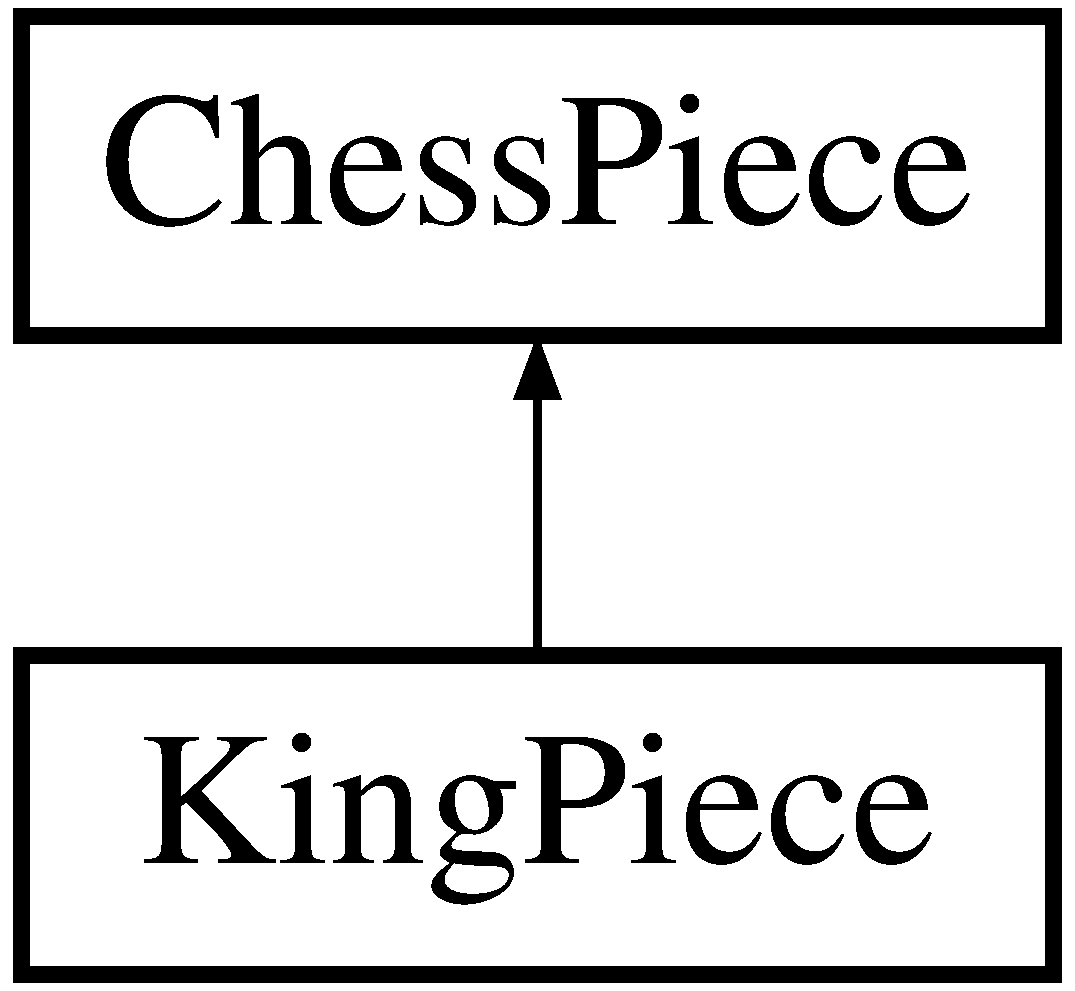
\includegraphics[height=2.000000cm]{class_king_piece}
\end{center}
\end{figure}
\subsection*{Public Member Functions}
\begin{DoxyCompactItemize}
\item 
\textbf{ King\+Piece} (class \textbf{ Chess\+Board} $\ast$a\+\_\+board, \textbf{ Position} a\+\_\+cell, \textbf{ Piece\+Color} a\+\_\+piece\+Color)
\begin{DoxyCompactList}\small\item\em King Piece Constructor. \end{DoxyCompactList}\item 
\textbf{ $\sim$\+King\+Piece} ()
\begin{DoxyCompactList}\small\item\em King Piece Desstructor. \end{DoxyCompactList}\item 
int \textbf{ move\+Piece} ()
\begin{DoxyCompactList}\small\item\em Overloaded move method to move King piece. \end{DoxyCompactList}\item 
\textbf{ Piece\+Type} \textbf{ get\+Piece\+Type} ()
\begin{DoxyCompactList}\small\item\em Return piece type. \end{DoxyCompactList}\item 
char \textbf{ piece\+Char\+Code} ()
\begin{DoxyCompactList}\small\item\em Return character representation of the king chess piece. \end{DoxyCompactList}\item 
std\+::vector$<$ \textbf{ Position} $>$ \textbf{ get\+Possible\+Moves} ()
\begin{DoxyCompactList}\small\item\em Get possible moves for the king piece. \end{DoxyCompactList}\end{DoxyCompactItemize}
\subsection*{Private Member Functions}
\begin{DoxyCompactItemize}
\item 
int \textbf{ distance\+To\+Rook} (std\+::vector$<$ \textbf{ Position} $>$ a\+\_\+possible\+Moves, \textbf{ Position} a\+\_\+pos\+Rook, \textbf{ Position} a\+\_\+pos\+King)
\begin{DoxyCompactList}\small\item\em Greedy method for Black King Piece to get the distance to the White Rook. \end{DoxyCompactList}\end{DoxyCompactItemize}
\subsection*{Additional Inherited Members}


\subsection{Detailed Description}
\doxyref{King\+Piece.\+hpp}{p.}{_king_piece_8hpp} \doxyref{King\+Piece}{p.}{class_king_piece} class. Inherits from \doxyref{Chess\+Piece}{p.}{class_chess_piece} class. Chess End Game Configurations.

Created by Salil Maharjan on 11/27/19. Copyright © 2019 Salil Maharjan. All rights reserved. 

\subsection{Constructor \& Destructor Documentation}
\mbox{\label{class_king_piece_afdd17637b739f79dc14215c31199d780}} 
\index{King\+Piece@{King\+Piece}!King\+Piece@{King\+Piece}}
\index{King\+Piece@{King\+Piece}!King\+Piece@{King\+Piece}}
\subsubsection{King\+Piece()}
{\footnotesize\ttfamily King\+Piece\+::\+King\+Piece (\begin{DoxyParamCaption}\item[{class \textbf{ Chess\+Board} $\ast$}]{a\+\_\+board,  }\item[{\textbf{ Position}}]{a\+\_\+cell,  }\item[{\textbf{ Piece\+Color}}]{a\+\_\+piece\+Color }\end{DoxyParamCaption})}



King Piece Constructor. 

\doxyref{King\+Piece.\+cpp}{p.}{_king_piece_8cpp} Implements \doxyref{King\+Piece.\+hpp}{p.}{_king_piece_8hpp} class. Chess End Game

Created by Salil Maharjan on 11/27/19. Copyright © 2019 Salil Maharjan. All rights reserved. King Piece class constructor. Constructor\+: Creates a \doxyref{King\+Piece}{p.}{class_king_piece} in a\+\_\+board chess board at cell position a\+\_\+cell. Calls \doxyref{Chess\+Piece}{p.}{class_chess_piece} constructor to construct a chesspiece. 
\begin{DoxyParams}{Parameters}
{\em a\+\_\+board} & Chess\+Board$\ast$ \doxyref{Chess\+Board}{p.}{class_chess_board} where the game is being played. \\
\hline
{\em a\+\_\+cell} & \doxyref{Position}{p.}{struct_position} (x,y) position to place king piece. \\
\hline
\end{DoxyParams}
\mbox{\label{class_king_piece_aae4567eac4bf9e4657215ca035271f76}} 
\index{King\+Piece@{King\+Piece}!````~King\+Piece@{$\sim$\+King\+Piece}}
\index{````~King\+Piece@{$\sim$\+King\+Piece}!King\+Piece@{King\+Piece}}
\subsubsection{$\sim$\+King\+Piece()}
{\footnotesize\ttfamily King\+Piece\+::$\sim$\+King\+Piece (\begin{DoxyParamCaption}{ }\end{DoxyParamCaption})}



King Piece Desstructor. 

King Piece class destructor. Destructor\+: Destroys the \doxyref{King\+Piece}{p.}{class_king_piece} from the board. 

\subsection{Member Function Documentation}
\mbox{\label{class_king_piece_a870c6bd42cf54b5e6c75044a8ffe7887}} 
\index{King\+Piece@{King\+Piece}!distance\+To\+Rook@{distance\+To\+Rook}}
\index{distance\+To\+Rook@{distance\+To\+Rook}!King\+Piece@{King\+Piece}}
\subsubsection{distance\+To\+Rook()}
{\footnotesize\ttfamily int King\+Piece\+::distance\+To\+Rook (\begin{DoxyParamCaption}\item[{std\+::vector$<$ \textbf{ Position} $>$}]{a\+\_\+possible\+Moves,  }\item[{\textbf{ Position}}]{a\+\_\+pos\+Rook,  }\item[{\textbf{ Position}}]{a\+\_\+pos\+King }\end{DoxyParamCaption})\hspace{0.3cm}{\ttfamily [private]}}



Greedy method for Black King Piece to get the distance to the White Rook. 

Greedy method for the Black King Piece. Used as a heuristic to select Black King move. Gets the distance from the Black King Piece to the White Rook Piece. Checks the minimum horizontal, vertical and diagonal distance, which is calculated using Euclidean distance, from the proposed position to the White Rook to get as close to it as possible. Also, as an improvement, checks the distance from the white king to see if there is a move so that it will get the Black Piece closer to the White Rook and away from the White King. At the end, the next move is chosen with the choice that has the most valid moves between the Rook\+Min\+Distance and King\+Max\+Distance. Priority given to getting close to the rook. So that it can eventually capture it without being on a check. 
\begin{DoxyParams}{Parameters}
{\em a\+\_\+pos\+Rook} & \doxyref{Position}{p.}{struct_position} The position of the White Rook. \\
\hline
{\em a\+\_\+pos\+King} & Possition The position of the White King. \\
\hline
\end{DoxyParams}
\begin{DoxyReturn}{Returns}
int The index of the best posssible move according to this greedy algorithm. 
\end{DoxyReturn}
\mbox{\label{class_king_piece_adf72b70a58939abb97041bf371184d59}} 
\index{King\+Piece@{King\+Piece}!get\+Piece\+Type@{get\+Piece\+Type}}
\index{get\+Piece\+Type@{get\+Piece\+Type}!King\+Piece@{King\+Piece}}
\subsubsection{get\+Piece\+Type()}
{\footnotesize\ttfamily \textbf{ Piece\+Type} King\+Piece\+::get\+Piece\+Type (\begin{DoxyParamCaption}{ }\end{DoxyParamCaption})\hspace{0.3cm}{\ttfamily [inline]}, {\ttfamily [virtual]}}



Return piece type. 



Implements \textbf{ Chess\+Piece} \doxyref{}{p.}{class_chess_piece_a3a0ae30c47fe6be0ed12859451a1e3f5}.

\mbox{\label{class_king_piece_ab1fc242e9d0c3bcace67a6839bf68cbd}} 
\index{King\+Piece@{King\+Piece}!get\+Possible\+Moves@{get\+Possible\+Moves}}
\index{get\+Possible\+Moves@{get\+Possible\+Moves}!King\+Piece@{King\+Piece}}
\subsubsection{get\+Possible\+Moves()}
{\footnotesize\ttfamily std\+::vector$<$ \textbf{ Position} $>$ King\+Piece\+::get\+Possible\+Moves (\begin{DoxyParamCaption}{ }\end{DoxyParamCaption})\hspace{0.3cm}{\ttfamily [virtual]}}



Get possible moves for the king piece. 

Method to get possible moves for a King Piece. \begin{DoxyReturn}{Returns}
vector$<$\+Position$>$ Array of possible positions the King piece can make a valid move to. 
\end{DoxyReturn}


Implements \textbf{ Chess\+Piece} \doxyref{}{p.}{class_chess_piece_a62e65eef509393e96e6122fd63e2915b}.

\mbox{\label{class_king_piece_a7c09258f545c61ad5323a14794f9eb66}} 
\index{King\+Piece@{King\+Piece}!move\+Piece@{move\+Piece}}
\index{move\+Piece@{move\+Piece}!King\+Piece@{King\+Piece}}
\subsubsection{move\+Piece()}
{\footnotesize\ttfamily int King\+Piece\+::move\+Piece (\begin{DoxyParamCaption}{ }\end{DoxyParamCaption})\hspace{0.3cm}{\ttfamily [virtual]}}



Overloaded move method to move King piece. 

Move method for King Piece. Overloaded move method to move King piece. \begin{DoxyReturn}{Returns}
int Returns 1 when the game ends due to checkmate and 2 when draw. 0 when in progress. 
\end{DoxyReturn}


Implements \textbf{ Chess\+Piece} \doxyref{}{p.}{class_chess_piece_aeed547e002595651caf20655a384d6e5}.

\mbox{\label{class_king_piece_af2bd66f1e7b5b8ab6ac29f930ea5e1fa}} 
\index{King\+Piece@{King\+Piece}!piece\+Char\+Code@{piece\+Char\+Code}}
\index{piece\+Char\+Code@{piece\+Char\+Code}!King\+Piece@{King\+Piece}}
\subsubsection{piece\+Char\+Code()}
{\footnotesize\ttfamily char King\+Piece\+::piece\+Char\+Code (\begin{DoxyParamCaption}{ }\end{DoxyParamCaption})\hspace{0.3cm}{\ttfamily [inline]}, {\ttfamily [virtual]}}



Return character representation of the king chess piece. 



Implements \textbf{ Chess\+Piece} \doxyref{}{p.}{class_chess_piece_ae07add53743a1fc66cdc92373d2dfe25}.



The documentation for this class was generated from the following files\+:\begin{DoxyCompactItemize}
\item 
chess\+End\+Game/\textbf{ King\+Piece.\+hpp}\item 
chess\+End\+Game/\textbf{ King\+Piece.\+cpp}\end{DoxyCompactItemize}

\section{Position Struct Reference}
\label{struct_position}\index{Position@{Position}}


\doxyref{Position}{p.}{struct_position} on the chess board.  




{\ttfamily \#include $<$Chess\+Piece.\+hpp$>$}

\subsection*{Public Attributes}
\begin{DoxyCompactItemize}
\item 
int \textbf{ x}
\item 
int \textbf{ y}
\end{DoxyCompactItemize}


\subsection{Detailed Description}
\doxyref{Position}{p.}{struct_position} on the chess board. 

\subsection{Member Data Documentation}
\mbox{\label{struct_position_aeda152ffeee17ae5be9c02327b2408d8}} 
\index{Position@{Position}!x@{x}}
\index{x@{x}!Position@{Position}}
\subsubsection{x}
{\footnotesize\ttfamily int Position\+::x}

\mbox{\label{struct_position_a3c08e9213d4726b21caba3073192c4a3}} 
\index{Position@{Position}!y@{y}}
\index{y@{y}!Position@{Position}}
\subsubsection{y}
{\footnotesize\ttfamily int Position\+::y}



The documentation for this struct was generated from the following file\+:\begin{DoxyCompactItemize}
\item 
chess\+End\+Game/\textbf{ Chess\+Piece.\+hpp}\end{DoxyCompactItemize}

\section{Rook\+Piece Class Reference}
\label{class_rook_piece}\index{Rook\+Piece@{Rook\+Piece}}


{\ttfamily \#include $<$Rook\+Piece.\+hpp$>$}

Inheritance diagram for Rook\+Piece\+:\begin{figure}[H]
\begin{center}
\leavevmode
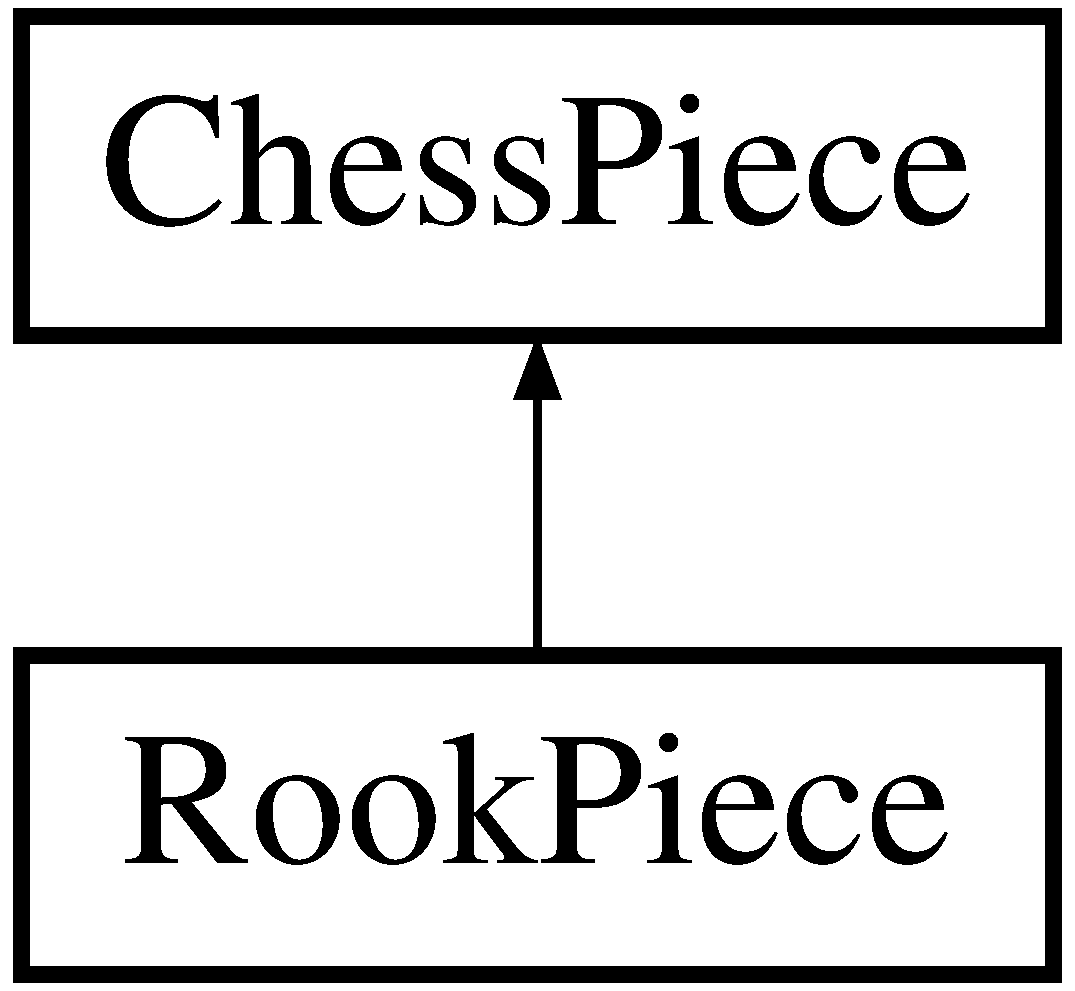
\includegraphics[height=2.000000cm]{class_rook_piece}
\end{center}
\end{figure}
\subsection*{Public Member Functions}
\begin{DoxyCompactItemize}
\item 
\textbf{ Rook\+Piece} (class \textbf{ Chess\+Board} $\ast$a\+\_\+board, \textbf{ Position} a\+\_\+cell, \textbf{ Piece\+Color} a\+\_\+piece\+Color)
\begin{DoxyCompactList}\small\item\em Rook Piece Constructor. \end{DoxyCompactList}\item 
\textbf{ $\sim$\+Rook\+Piece} ()
\begin{DoxyCompactList}\small\item\em Rook Piece Desstructor. \end{DoxyCompactList}\item 
int \textbf{ move\+Piece} ()
\begin{DoxyCompactList}\small\item\em Overloaded move method to move Rook piece. \end{DoxyCompactList}\item 
\textbf{ Piece\+Type} \textbf{ get\+Piece\+Type} ()
\begin{DoxyCompactList}\small\item\em Return piece type. \end{DoxyCompactList}\item 
char \textbf{ piece\+Char\+Code} ()
\begin{DoxyCompactList}\small\item\em Return character representation of the king chess piece. \end{DoxyCompactList}\item 
std\+::vector$<$ \textbf{ Position} $>$ \textbf{ get\+Possible\+Moves} ()
\begin{DoxyCompactList}\small\item\em Get possible moves for the rook. \end{DoxyCompactList}\end{DoxyCompactItemize}
\subsection*{Private Member Functions}
\begin{DoxyCompactItemize}
\item 
bool \textbf{ check\+Path} (\textbf{ Position} a\+\_\+current, \textbf{ Position} a\+\_\+pos)
\begin{DoxyCompactList}\small\item\em Method to check path of the Rook if there are obstructions. \end{DoxyCompactList}\end{DoxyCompactItemize}
\subsection*{Additional Inherited Members}


\subsection{Detailed Description}
\doxyref{Rook\+Piece.\+hpp}{p.}{_rook_piece_8hpp} \doxyref{Rook\+Piece}{p.}{class_rook_piece} class. Inherits from \doxyref{Chess\+Piece}{p.}{class_chess_piece} class. Chess End Game Configurations.

Created by Salil Maharjan on 11/27/19. Copyright © 2019 Salil Maharjan. All rights reserved. 

\subsection{Constructor \& Destructor Documentation}
\mbox{\label{class_rook_piece_acc4f433e6ed23cd60457caa031be51f0}} 
\index{Rook\+Piece@{Rook\+Piece}!Rook\+Piece@{Rook\+Piece}}
\index{Rook\+Piece@{Rook\+Piece}!Rook\+Piece@{Rook\+Piece}}
\subsubsection{Rook\+Piece()}
{\footnotesize\ttfamily Rook\+Piece\+::\+Rook\+Piece (\begin{DoxyParamCaption}\item[{class \textbf{ Chess\+Board} $\ast$}]{a\+\_\+board,  }\item[{\textbf{ Position}}]{a\+\_\+cell,  }\item[{\textbf{ Piece\+Color}}]{a\+\_\+piece\+Color }\end{DoxyParamCaption})}



Rook Piece Constructor. 

\doxyref{Rook\+Piece.\+cpp}{p.}{_rook_piece_8cpp} Implements \doxyref{Rook\+Piece.\+hpp}{p.}{_rook_piece_8hpp} class. Chess End Game

Created by Salil Maharjan on 11/27/19. Copyright © 2019 Salil Maharjan. All rights reserved. Rook Piece class constructor. Constructor\+: Creates a \doxyref{Rook\+Piece}{p.}{class_rook_piece} in a\+\_\+board chess board at cell position a\+\_\+cell. Calls \doxyref{Chess\+Piece}{p.}{class_chess_piece} constructor to construct a chesspiece. 
\begin{DoxyParams}{Parameters}
{\em a\+\_\+board} & Chess\+Board$\ast$ \doxyref{Chess\+Board}{p.}{class_chess_board} where the game is being played. \\
\hline
{\em a\+\_\+cell} & \doxyref{Position}{p.}{struct_position} (x,y) position to place king piece. \\
\hline
\end{DoxyParams}
\mbox{\label{class_rook_piece_a5907779639688e58f4b50eb4eca4ebb1}} 
\index{Rook\+Piece@{Rook\+Piece}!````~Rook\+Piece@{$\sim$\+Rook\+Piece}}
\index{````~Rook\+Piece@{$\sim$\+Rook\+Piece}!Rook\+Piece@{Rook\+Piece}}
\subsubsection{$\sim$\+Rook\+Piece()}
{\footnotesize\ttfamily Rook\+Piece\+::$\sim$\+Rook\+Piece (\begin{DoxyParamCaption}{ }\end{DoxyParamCaption})}



Rook Piece Desstructor. 

Rook Piece class destructor. Destructor\+: Destroys the rook piece from the board. 

\subsection{Member Function Documentation}
\mbox{\label{class_rook_piece_ae4272efa6dc5a3ee6ffea5af987a65f1}} 
\index{Rook\+Piece@{Rook\+Piece}!check\+Path@{check\+Path}}
\index{check\+Path@{check\+Path}!Rook\+Piece@{Rook\+Piece}}
\subsubsection{check\+Path()}
{\footnotesize\ttfamily bool Rook\+Piece\+::check\+Path (\begin{DoxyParamCaption}\item[{\textbf{ Position}}]{a\+\_\+current,  }\item[{\textbf{ Position}}]{a\+\_\+pos }\end{DoxyParamCaption})\hspace{0.3cm}{\ttfamily [private]}}



Method to check path of the Rook if there are obstructions. 

Method to check path of the Rook if there are obstructions. Returns a bool depending on if there are obstructions on the path of the Rook or not. 
\begin{DoxyParams}{Parameters}
{\em a\+\_\+current} & \doxyref{Position}{p.}{struct_position} Current position of the Rook \\
\hline
{\em a\+\_\+pos} & \doxyref{Position}{p.}{struct_position} The rook\textquotesingle{}s destination position. \\
\hline
\end{DoxyParams}
\begin{DoxyReturn}{Returns}
bool True if there are no obstructions and the rook can move, false otherwise. 
\end{DoxyReturn}
\mbox{\label{class_rook_piece_addfa6bc37715d63b05e96f5fbd5a26ab}} 
\index{Rook\+Piece@{Rook\+Piece}!get\+Piece\+Type@{get\+Piece\+Type}}
\index{get\+Piece\+Type@{get\+Piece\+Type}!Rook\+Piece@{Rook\+Piece}}
\subsubsection{get\+Piece\+Type()}
{\footnotesize\ttfamily \textbf{ Piece\+Type} Rook\+Piece\+::get\+Piece\+Type (\begin{DoxyParamCaption}{ }\end{DoxyParamCaption})\hspace{0.3cm}{\ttfamily [inline]}, {\ttfamily [virtual]}}



Return piece type. 



Implements \textbf{ Chess\+Piece} \doxyref{}{p.}{class_chess_piece_a3a0ae30c47fe6be0ed12859451a1e3f5}.

\mbox{\label{class_rook_piece_afffc17359851023ef3db115c9ff50680}} 
\index{Rook\+Piece@{Rook\+Piece}!get\+Possible\+Moves@{get\+Possible\+Moves}}
\index{get\+Possible\+Moves@{get\+Possible\+Moves}!Rook\+Piece@{Rook\+Piece}}
\subsubsection{get\+Possible\+Moves()}
{\footnotesize\ttfamily std\+::vector$<$ \textbf{ Position} $>$ Rook\+Piece\+::get\+Possible\+Moves (\begin{DoxyParamCaption}{ }\end{DoxyParamCaption})\hspace{0.3cm}{\ttfamily [virtual]}}



Get possible moves for the rook. 

Method to get possible moves for a Rook Piece. \begin{DoxyReturn}{Returns}
vector$<$\+Position$>$ Array of possible positions the Rook piece can make a valid move to. 
\end{DoxyReturn}


Implements \textbf{ Chess\+Piece} \doxyref{}{p.}{class_chess_piece_a62e65eef509393e96e6122fd63e2915b}.

\mbox{\label{class_rook_piece_a083ee01e8799014bcf7d36968b008386}} 
\index{Rook\+Piece@{Rook\+Piece}!move\+Piece@{move\+Piece}}
\index{move\+Piece@{move\+Piece}!Rook\+Piece@{Rook\+Piece}}
\subsubsection{move\+Piece()}
{\footnotesize\ttfamily int Rook\+Piece\+::move\+Piece (\begin{DoxyParamCaption}{ }\end{DoxyParamCaption})\hspace{0.3cm}{\ttfamily [virtual]}}



Overloaded move method to move Rook piece. 

Move method for Rook Piece. Overloaded move method to move Rook piece. 

Implements \textbf{ Chess\+Piece} \doxyref{}{p.}{class_chess_piece_aeed547e002595651caf20655a384d6e5}.

\mbox{\label{class_rook_piece_a163839b3da6d698e77267f18f72a2383}} 
\index{Rook\+Piece@{Rook\+Piece}!piece\+Char\+Code@{piece\+Char\+Code}}
\index{piece\+Char\+Code@{piece\+Char\+Code}!Rook\+Piece@{Rook\+Piece}}
\subsubsection{piece\+Char\+Code()}
{\footnotesize\ttfamily char Rook\+Piece\+::piece\+Char\+Code (\begin{DoxyParamCaption}{ }\end{DoxyParamCaption})\hspace{0.3cm}{\ttfamily [inline]}, {\ttfamily [virtual]}}



Return character representation of the king chess piece. 



Implements \textbf{ Chess\+Piece} \doxyref{}{p.}{class_chess_piece_ae07add53743a1fc66cdc92373d2dfe25}.



The documentation for this class was generated from the following files\+:\begin{DoxyCompactItemize}
\item 
chess\+End\+Game/\textbf{ Rook\+Piece.\+hpp}\item 
chess\+End\+Game/\textbf{ Rook\+Piece.\+cpp}\end{DoxyCompactItemize}

\chapter{File Documentation}
\section{chess\+End\+Game/\+Chess\+Board.cpp File Reference}
\label{_chess_board_8cpp}\index{chess\+End\+Game/\+Chess\+Board.\+cpp@{chess\+End\+Game/\+Chess\+Board.\+cpp}}
{\ttfamily \#include \char`\"{}Chess\+Board.\+hpp\char`\"{}}\newline
{\ttfamily \#include \char`\"{}King\+Piece.\+hpp\char`\"{}}\newline
{\ttfamily \#include \char`\"{}Rook\+Piece.\+hpp\char`\"{}}\newline
{\ttfamily \#include \char`\"{}Global\+Counter.\+hpp\char`\"{}}\newline
{\ttfamily \#include $<$iostream$>$}\newline
{\ttfamily \#include $<$iomanip$>$}\newline
{\ttfamily \#include $<$fstream$>$}\newline
\subsection*{Variables}
\begin{DoxyCompactItemize}
\item 
std\+::ofstream \textbf{ write\+File}
\end{DoxyCompactItemize}


\subsection{Variable Documentation}
\mbox{\label{_chess_board_8cpp_a8ffd7986de49cea6d16362f73a7d9d00}} 
\index{Chess\+Board.\+cpp@{Chess\+Board.\+cpp}!write\+File@{write\+File}}
\index{write\+File@{write\+File}!Chess\+Board.\+cpp@{Chess\+Board.\+cpp}}
\subsubsection{write\+File}
{\footnotesize\ttfamily std\+::ofstream write\+File}

\doxyref{Chess\+Board.\+cpp}{p.}{_chess_board_8cpp} Implementation of \doxyref{Chess\+Board.\+hpp}{p.}{_chess_board_8hpp} class.

Created by Salil D. Maharjan on 11/27/19. Copyright © 2019 Salil Maharjan. All rights reserved. 
\section{chess\+End\+Game/\+Chess\+Board.hpp File Reference}
\label{_chess_board_8hpp}\index{chess\+End\+Game/\+Chess\+Board.\+hpp@{chess\+End\+Game/\+Chess\+Board.\+hpp}}
{\ttfamily \#include \char`\"{}Chess\+Piece.\+hpp\char`\"{}}\newline
{\ttfamily \#include $<$stdio.\+h$>$}\newline
\subsection*{Classes}
\begin{DoxyCompactItemize}
\item 
class \textbf{ Chess\+Board}
\begin{DoxyCompactList}\small\item\em Singleton Board Class. \end{DoxyCompactList}\end{DoxyCompactItemize}

\section{chess\+End\+Game/\+Chess\+Piece.cpp File Reference}
\label{_chess_piece_8cpp}\index{chess\+End\+Game/\+Chess\+Piece.\+cpp@{chess\+End\+Game/\+Chess\+Piece.\+cpp}}
{\ttfamily \#include $<$iostream$>$}\newline
{\ttfamily \#include \char`\"{}Chess\+Piece.\+hpp\char`\"{}}\newline
{\ttfamily \#include \char`\"{}Chess\+Board.\+hpp\char`\"{}}\newline
{\ttfamily \#include \char`\"{}Global\+Counter.\+hpp\char`\"{}}\newline

\section{chess\+End\+Game/\+Chess\+Piece.hpp File Reference}
\label{_chess_piece_8hpp}\index{chess\+End\+Game/\+Chess\+Piece.\+hpp@{chess\+End\+Game/\+Chess\+Piece.\+hpp}}
{\ttfamily \#include $<$stdio.\+h$>$}\newline
{\ttfamily \#include $<$vector$>$}\newline
\subsection*{Classes}
\begin{DoxyCompactItemize}
\item 
struct \textbf{ Position}
\begin{DoxyCompactList}\small\item\em \doxyref{Position}{p.}{struct_position} on the chess board. \end{DoxyCompactList}\item 
class \textbf{ Chess\+Piece}
\end{DoxyCompactItemize}
\subsection*{Macros}
\begin{DoxyCompactItemize}
\item 
\#define \textbf{ Chess\+Piece\+\_\+hpp}
\end{DoxyCompactItemize}
\subsection*{Enumerations}
\begin{DoxyCompactItemize}
\item 
enum \textbf{ Piece\+Type} \{ \textbf{ K\+I\+NG}, 
\textbf{ R\+O\+OK}
 \}
\begin{DoxyCompactList}\small\item\em Chess piece type. \end{DoxyCompactList}\item 
enum \textbf{ Piece\+Color} \{ \textbf{ B\+L\+A\+CK}, 
\textbf{ W\+H\+I\+TE}
 \}
\begin{DoxyCompactList}\small\item\em Chess color type. \end{DoxyCompactList}\end{DoxyCompactItemize}


\subsection{Macro Definition Documentation}
\mbox{\label{_chess_piece_8hpp_a473776fad278bca0eebd32c879118eeb}} 
\index{Chess\+Piece.\+hpp@{Chess\+Piece.\+hpp}!Chess\+Piece\+\_\+hpp@{Chess\+Piece\+\_\+hpp}}
\index{Chess\+Piece\+\_\+hpp@{Chess\+Piece\+\_\+hpp}!Chess\+Piece.\+hpp@{Chess\+Piece.\+hpp}}
\subsubsection{Chess\+Piece\+\_\+hpp}
{\footnotesize\ttfamily \#define Chess\+Piece\+\_\+hpp}

\doxyref{Chess\+Piece.\+hpp}{p.}{_chess_piece_8hpp} \doxyref{Chess\+Piece}{p.}{class_chess_piece} Class header file. Class that implementss chess pieces.

Created by Salil Maharjan on 11/27/19. Copyright © 2019 Salil Maharjan. All rights reserved. 

\subsection{Enumeration Type Documentation}
\mbox{\label{_chess_piece_8hpp_ad7595c48bb74c0dd2a7648712a2d4985}} 
\index{Chess\+Piece.\+hpp@{Chess\+Piece.\+hpp}!Piece\+Color@{Piece\+Color}}
\index{Piece\+Color@{Piece\+Color}!Chess\+Piece.\+hpp@{Chess\+Piece.\+hpp}}
\subsubsection{Piece\+Color}
{\footnotesize\ttfamily enum \textbf{ Piece\+Color}}



Chess color type. 

\begin{DoxyEnumFields}{Enumerator}
\raisebox{\heightof{T}}[0pt][0pt]{\index{B\+L\+A\+CK@{B\+L\+A\+CK}!Chess\+Piece.\+hpp@{Chess\+Piece.\+hpp}}\index{Chess\+Piece.\+hpp@{Chess\+Piece.\+hpp}!B\+L\+A\+CK@{B\+L\+A\+CK}}}\mbox{\label{_chess_piece_8hpp_ad7595c48bb74c0dd2a7648712a2d4985af77fb67151d0c18d397069ad8c271ba3}} 
B\+L\+A\+CK&\\
\hline

\raisebox{\heightof{T}}[0pt][0pt]{\index{W\+H\+I\+TE@{W\+H\+I\+TE}!Chess\+Piece.\+hpp@{Chess\+Piece.\+hpp}}\index{Chess\+Piece.\+hpp@{Chess\+Piece.\+hpp}!W\+H\+I\+TE@{W\+H\+I\+TE}}}\mbox{\label{_chess_piece_8hpp_ad7595c48bb74c0dd2a7648712a2d4985a283fc479650da98250635b9c3c0e7e50}} 
W\+H\+I\+TE&\\
\hline

\end{DoxyEnumFields}
\mbox{\label{_chess_piece_8hpp_a12ed9719bbdf7bc596ff7a6f4bf3f021}} 
\index{Chess\+Piece.\+hpp@{Chess\+Piece.\+hpp}!Piece\+Type@{Piece\+Type}}
\index{Piece\+Type@{Piece\+Type}!Chess\+Piece.\+hpp@{Chess\+Piece.\+hpp}}
\subsubsection{Piece\+Type}
{\footnotesize\ttfamily enum \textbf{ Piece\+Type}}



Chess piece type. 

\begin{DoxyEnumFields}{Enumerator}
\raisebox{\heightof{T}}[0pt][0pt]{\index{K\+I\+NG@{K\+I\+NG}!Chess\+Piece.\+hpp@{Chess\+Piece.\+hpp}}\index{Chess\+Piece.\+hpp@{Chess\+Piece.\+hpp}!K\+I\+NG@{K\+I\+NG}}}\mbox{\label{_chess_piece_8hpp_a12ed9719bbdf7bc596ff7a6f4bf3f021a157524408d6f0fc4b7dc5e52f3dd3b80}} 
K\+I\+NG&\\
\hline

\raisebox{\heightof{T}}[0pt][0pt]{\index{R\+O\+OK@{R\+O\+OK}!Chess\+Piece.\+hpp@{Chess\+Piece.\+hpp}}\index{Chess\+Piece.\+hpp@{Chess\+Piece.\+hpp}!R\+O\+OK@{R\+O\+OK}}}\mbox{\label{_chess_piece_8hpp_a12ed9719bbdf7bc596ff7a6f4bf3f021a49b75ad9a5137e805c60f32ed9cc2820}} 
R\+O\+OK&\\
\hline

\end{DoxyEnumFields}

\section{chess\+End\+Game/\+Global\+Counter.cpp File Reference}
\label{_global_counter_8cpp}\index{chess\+End\+Game/\+Global\+Counter.\+cpp@{chess\+End\+Game/\+Global\+Counter.\+cpp}}
{\ttfamily \#include \char`\"{}Global\+Counter.\+hpp\char`\"{}}\newline
\subsection*{Variables}
\begin{DoxyCompactItemize}
\item 
int \textbf{ g\+\_\+white\+State\+Counter} = 0
\item 
int \textbf{ g\+\_\+black\+State\+Counter} = 0
\end{DoxyCompactItemize}


\subsection{Variable Documentation}
\mbox{\label{_global_counter_8cpp_a1f9bf1d82001608d9893e2c948017fe8}} 
\index{Global\+Counter.\+cpp@{Global\+Counter.\+cpp}!g\+\_\+black\+State\+Counter@{g\+\_\+black\+State\+Counter}}
\index{g\+\_\+black\+State\+Counter@{g\+\_\+black\+State\+Counter}!Global\+Counter.\+cpp@{Global\+Counter.\+cpp}}
\subsubsection{g\+\_\+black\+State\+Counter}
{\footnotesize\ttfamily int g\+\_\+black\+State\+Counter = 0}

\mbox{\label{_global_counter_8cpp_ab0ab212cda0979165ed2f280a9e7c7fe}} 
\index{Global\+Counter.\+cpp@{Global\+Counter.\+cpp}!g\+\_\+white\+State\+Counter@{g\+\_\+white\+State\+Counter}}
\index{g\+\_\+white\+State\+Counter@{g\+\_\+white\+State\+Counter}!Global\+Counter.\+cpp@{Global\+Counter.\+cpp}}
\subsubsection{g\+\_\+white\+State\+Counter}
{\footnotesize\ttfamily int g\+\_\+white\+State\+Counter = 0}

\doxyref{Global\+Counter.\+cpp}{p.}{_global_counter_8cpp} Implementation of \doxyref{Global\+Counter.\+hpp}{p.}{_global_counter_8hpp} class.

Created by Salil D. Maharjan on 12/10/19. Copyright © 2019 Salil Maharjan. All rights reserved. 
\section{chess\+End\+Game/\+Global\+Counter.hpp File Reference}
\label{_global_counter_8hpp}\index{chess\+End\+Game/\+Global\+Counter.\+hpp@{chess\+End\+Game/\+Global\+Counter.\+hpp}}
{\ttfamily \#include $<$stdio.\+h$>$}\newline
\subsection*{Variables}
\begin{DoxyCompactItemize}
\item 
int \textbf{ g\+\_\+white\+State\+Counter}
\item 
int \textbf{ g\+\_\+black\+State\+Counter}
\end{DoxyCompactItemize}


\subsection{Variable Documentation}
\mbox{\label{_global_counter_8hpp_a1f9bf1d82001608d9893e2c948017fe8}} 
\index{Global\+Counter.\+hpp@{Global\+Counter.\+hpp}!g\+\_\+black\+State\+Counter@{g\+\_\+black\+State\+Counter}}
\index{g\+\_\+black\+State\+Counter@{g\+\_\+black\+State\+Counter}!Global\+Counter.\+hpp@{Global\+Counter.\+hpp}}
\subsubsection{g\+\_\+black\+State\+Counter}
{\footnotesize\ttfamily int g\+\_\+black\+State\+Counter}

\mbox{\label{_global_counter_8hpp_ab0ab212cda0979165ed2f280a9e7c7fe}} 
\index{Global\+Counter.\+hpp@{Global\+Counter.\+hpp}!g\+\_\+white\+State\+Counter@{g\+\_\+white\+State\+Counter}}
\index{g\+\_\+white\+State\+Counter@{g\+\_\+white\+State\+Counter}!Global\+Counter.\+hpp@{Global\+Counter.\+hpp}}
\subsubsection{g\+\_\+white\+State\+Counter}
{\footnotesize\ttfamily int g\+\_\+white\+State\+Counter}

\doxyref{Global\+Counter.\+hpp}{p.}{_global_counter_8hpp} Global Counter Class header. Class that implementss a global counter to keep track of states visited in alpha beta and greedy algorithm.

Created by Salil Maharjan on 11/27/19. Copyright © 2019 Salil Maharjan. All rights reserved.

\doxyref{Global\+Counter.\+cpp}{p.}{_global_counter_8cpp} Implementation of \doxyref{Global\+Counter.\+hpp}{p.}{_global_counter_8hpp} class.

Created by Salil D. Maharjan on 12/10/19. Copyright © 2019 Salil Maharjan. All rights reserved. 
\section{chess\+End\+Game/\+King\+Piece.cpp File Reference}
\label{_king_piece_8cpp}\index{chess\+End\+Game/\+King\+Piece.\+cpp@{chess\+End\+Game/\+King\+Piece.\+cpp}}
{\ttfamily \#include $<$iostream$>$}\newline
{\ttfamily \#include $<$cmath$>$}\newline
{\ttfamily \#include \char`\"{}King\+Piece.\+hpp\char`\"{}}\newline
{\ttfamily \#include \char`\"{}Chess\+Piece.\+hpp\char`\"{}}\newline
{\ttfamily \#include \char`\"{}Global\+Counter.\+hpp\char`\"{}}\newline

\section{chess\+End\+Game/\+King\+Piece.hpp File Reference}
\label{_king_piece_8hpp}\index{chess\+End\+Game/\+King\+Piece.\+hpp@{chess\+End\+Game/\+King\+Piece.\+hpp}}
{\ttfamily \#include $<$stdio.\+h$>$}\newline
{\ttfamily \#include \char`\"{}Chess\+Board.\+hpp\char`\"{}}\newline
{\ttfamily \#include \char`\"{}Chess\+Piece.\+hpp\char`\"{}}\newline
\subsection*{Classes}
\begin{DoxyCompactItemize}
\item 
class \textbf{ King\+Piece}
\end{DoxyCompactItemize}

\section{chess\+End\+Game/main.cpp File Reference}
\label{main_8cpp}\index{chess\+End\+Game/main.\+cpp@{chess\+End\+Game/main.\+cpp}}
{\ttfamily \#include $<$iostream$>$}\newline
{\ttfamily \#include $<$fstream$>$}\newline
{\ttfamily \#include \char`\"{}Chess\+Board.\+hpp\char`\"{}}\newline
{\ttfamily \#include \char`\"{}Global\+Counter.\+hpp\char`\"{}}\newline
\subsection*{Functions}
\begin{DoxyCompactItemize}
\item 
int \textbf{ main} (int argc, const char $\ast$argv[$\,$])
\end{DoxyCompactItemize}


\subsection{Function Documentation}
\mbox{\label{main_8cpp_ac0f2228420376f4db7e1274f2b41667c}} 
\index{main.\+cpp@{main.\+cpp}!main@{main}}
\index{main@{main}!main.\+cpp@{main.\+cpp}}
\subsubsection{main()}
{\footnotesize\ttfamily int main (\begin{DoxyParamCaption}\item[{int}]{argc,  }\item[{const char $\ast$}]{argv[$\,$] }\end{DoxyParamCaption})}

\doxyref{main.\+cpp}{p.}{main_8cpp} Main for the Chess End Game Configurations Project. Defines the entry point.

Created by Salil Maharjan on 11/27/19. Copyright © 2019 Salil Maharjan. All rights reserved. 
\section{chess\+End\+Game/\+Rook\+Piece.cpp File Reference}
\label{_rook_piece_8cpp}\index{chess\+End\+Game/\+Rook\+Piece.\+cpp@{chess\+End\+Game/\+Rook\+Piece.\+cpp}}
{\ttfamily \#include $<$iostream$>$}\newline
{\ttfamily \#include \char`\"{}Rook\+Piece.\+hpp\char`\"{}}\newline
{\ttfamily \#include \char`\"{}Chess\+Piece.\+hpp\char`\"{}}\newline
{\ttfamily \#include \char`\"{}Global\+Counter.\+hpp\char`\"{}}\newline

\section{chess\+End\+Game/\+Rook\+Piece.hpp File Reference}
\label{_rook_piece_8hpp}\index{chess\+End\+Game/\+Rook\+Piece.\+hpp@{chess\+End\+Game/\+Rook\+Piece.\+hpp}}
{\ttfamily \#include $<$stdio.\+h$>$}\newline
{\ttfamily \#include \char`\"{}Chess\+Board.\+hpp\char`\"{}}\newline
{\ttfamily \#include \char`\"{}Chess\+Piece.\+hpp\char`\"{}}\newline
\subsection*{Classes}
\begin{DoxyCompactItemize}
\item 
class \textbf{ Rook\+Piece}
\end{DoxyCompactItemize}

%--- End generated contents ---

% Index
\backmatter
\newpage
\phantomsection
\clearemptydoublepage
\addcontentsline{toc}{chapter}{Index}
\printindex

\end{document}
